\documentclass[Report.tex]{subfiles}
\begin{document}
This section describes the typical work flow of a data scientist. We will focus on the following four faces: Preparation, Analysis, Reflection and Dissemination.

The process of getting the data, understanding the data and produce results is an iterative process. The process is seen on Figure \ref{Fig:Iterative}.

\begin{figure}
\center
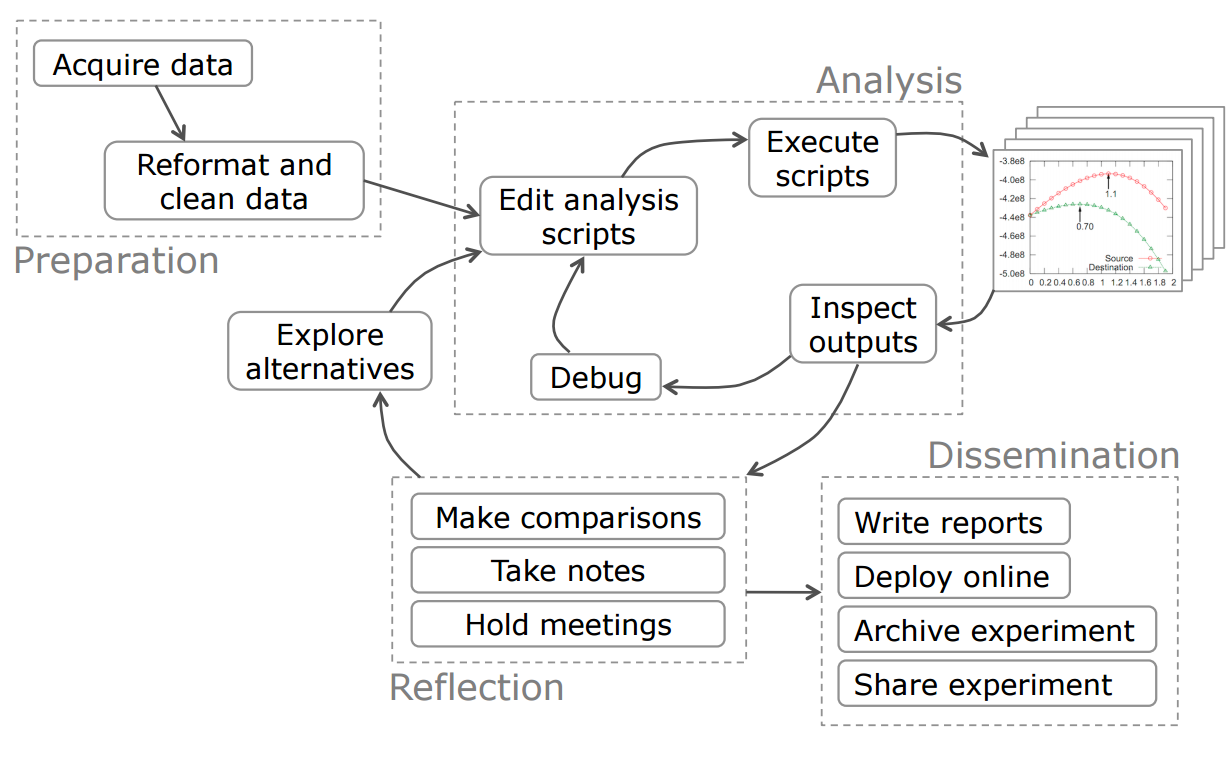
\includegraphics[scale=0.4]{Iterative.png}
\caption{The model showing the iterative process\cite[Chapter 2]{Guo}}
\label{Fig:Iterative}
\end{figure}
\begin{itemize}


\item The first face is the preparation face. Here the you have to acquire the data, that could be from hard disks, servers, through an API ect. Where to store and how to organize the data files should be considered, so it is easy to replace the right files if the data gets updated. Then the data should be cleaned, meaning removing tuples with missing values, changing the formatting, sorting the data ect.


\item The second face is the analysis face. Here the data is analysed to get more information about it. This is an iterative process, where the you create and run scripts,  look at the output, maybe find some mistakes, debug these and run it again. 

\item The third face is the reflection face. Here the output results is discussed, for example by making comparisons between outputs, and exploring alternatives.

\item The fourth and last face is the dissemination face. Here the the results are reported and maybe published in a report.
\cite[Chapter 2]{Guo}


\end{itemize}

\end{document}